\documentclass{article}
\usepackage{tikz}
\usetikzlibrary{mindmap} % LATEX and plain TEX when using TikZ
\begin{document}
\tikz[mindmap,concept color=red!50]
\node [concept] {Root concept}
child[grow=right] {node[concept] {Child concept}};

\tikz[large mindmap,concept color=red!50]
\node [concept] {Root concept}
child[grow=right] {node[concept] {Child concept}};

\tikz[mindmap,concept color=red!50] \node [concept] {Some concept};

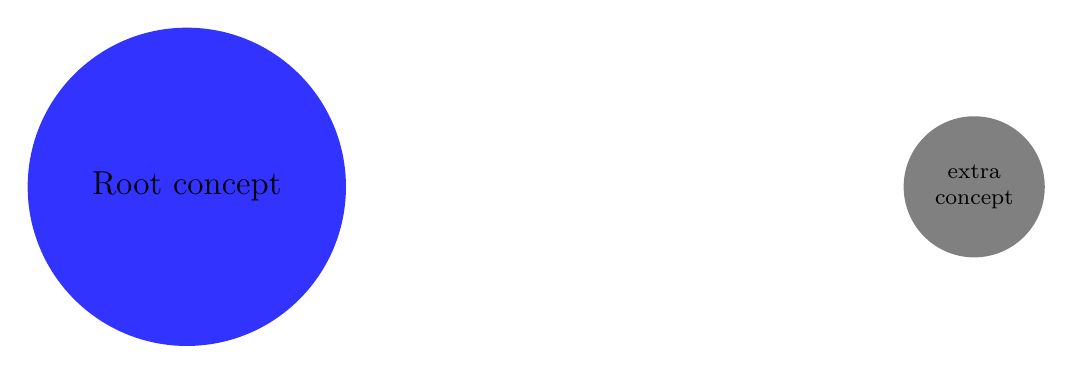
\begin{tikzpicture}[mindmap,concept color=blue!80]
\node [concept] {Root concept};
\node [extra concept] at (10,0) {extra concept};
\end{tikzpicture}

\tikz[root concept/.append style={concept color=blue!80,minimum size=3.5cm},mindmap]
\node [concept] {Root concept};

\tikz[root concept/.append style={concept color=blue!80},level 1 concept/.append style={concept color=red!50},mindmap]
\node [concept] {Root concept}
    child[grow=30] {node[concept] {child}}
    child[grow=0 ] {node[concept] {child}};
    
\tikz[mindmap,concept color=blue!80]
\node [concept] {Root concept}
child[concept color=red,grow=30] {node[concept] {Child concept}}
child[concept color=orange,grow=0] {node[concept] {Child concept}};

\tikz[mindmap,text=white,
root concept/.style={concept color=blue},
level 1 concept/.append style=
{every child/.style={concept color=blue!50}}]
\node [concept] {Root concept}
child[grow=30] {node[concept] {child}}
child[grow=0 ] {node[concept] {child}};

% \begin{tikzpicture}
% [root concept/.append style={concept color=blue!20,minimum size=2cm},
% level 1 concept/.append style={sibling angle=45},
% mindmap]
% \node [concept] {Root concept}
% [clockwise from=45]
% child { node[concept] (c1) {child}}
% child { node[concept] (c2) {child}}
% child { node[concept] (c3) {child}};
% \begin{pgfonlayer}{background}
% \draw [concept connection] (c1) edge (c2)
% edge (c3)
% (c2) edge (c3);
% \end{pgfonlayer}
% \end{tikzpicture}

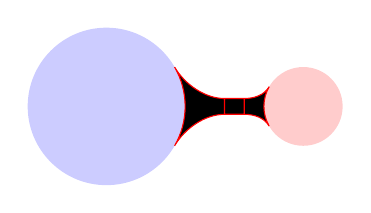
\begin{tikzpicture}
[decoration={start radius=1cm,end radius=.5cm,amplitude=2mm,angle=30}]
\fill[blue!20] (0,0) circle (1cm);
\fill[red!20] (2.5,0) circle (.5cm);
\filldraw [draw=red,fill=black,
decorate,decoration=circle connection bar] (1,0) -- (2,0);
\end{tikzpicture}

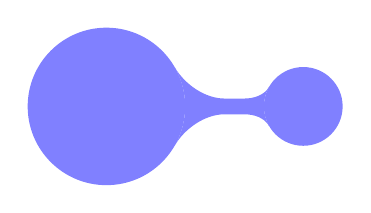
\begin{tikzpicture}
[blue!50,decoration={start radius=1cm,
end radius=.5cm,amplitude=2mm,angle=30}]
\fill (0,0) circle (1cm);
\fill (2.5,0) circle (.5cm);
\fill [decorate,decoration=circle connection bar] (1,0) -- (2,0);
\end{tikzpicture}

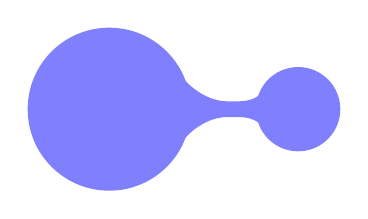
\begin{tikzpicture}
[blue!50,decoration={start radius=1cm,
end radius=.5cm,amplitude=2mm,angle=30}]
\fill (0,0) circle (1cm+1pt);
\fill (2.4,0) circle (.5cm+1pt);
\fill [decorate,decoration=circle connection bar] (1,0) -- (1.9,0);
\end{tikzpicture}

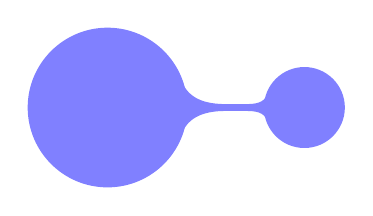
\begin{tikzpicture}[concept color=blue!50,blue!50,outer sep=0pt]
\node (n1) at (0,0) [circle,minimum size=2cm,fill,draw,thick] {};
\node (n2) at (2.5,0) [circle,minimum size=1cm,fill,draw,thick] {};
\path (n1) to[circle connection bar] (n2);
\end{tikzpicture}

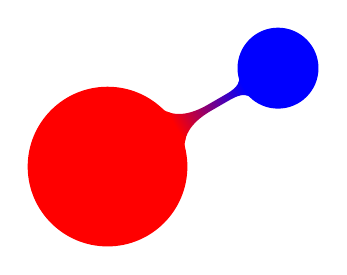
\begin{tikzpicture}[outer sep=0pt]
\node (n1) at (0,0) [circle,minimum size=2cm,fill,draw,thick,red] {};
\node (n2) at (30:2.5) [circle,minimum size=1cm,fill,draw,thick,blue] {};
\path (n1) to[circle connection bar switch color=from (red) to (blue)] (n2);
\end{tikzpicture}

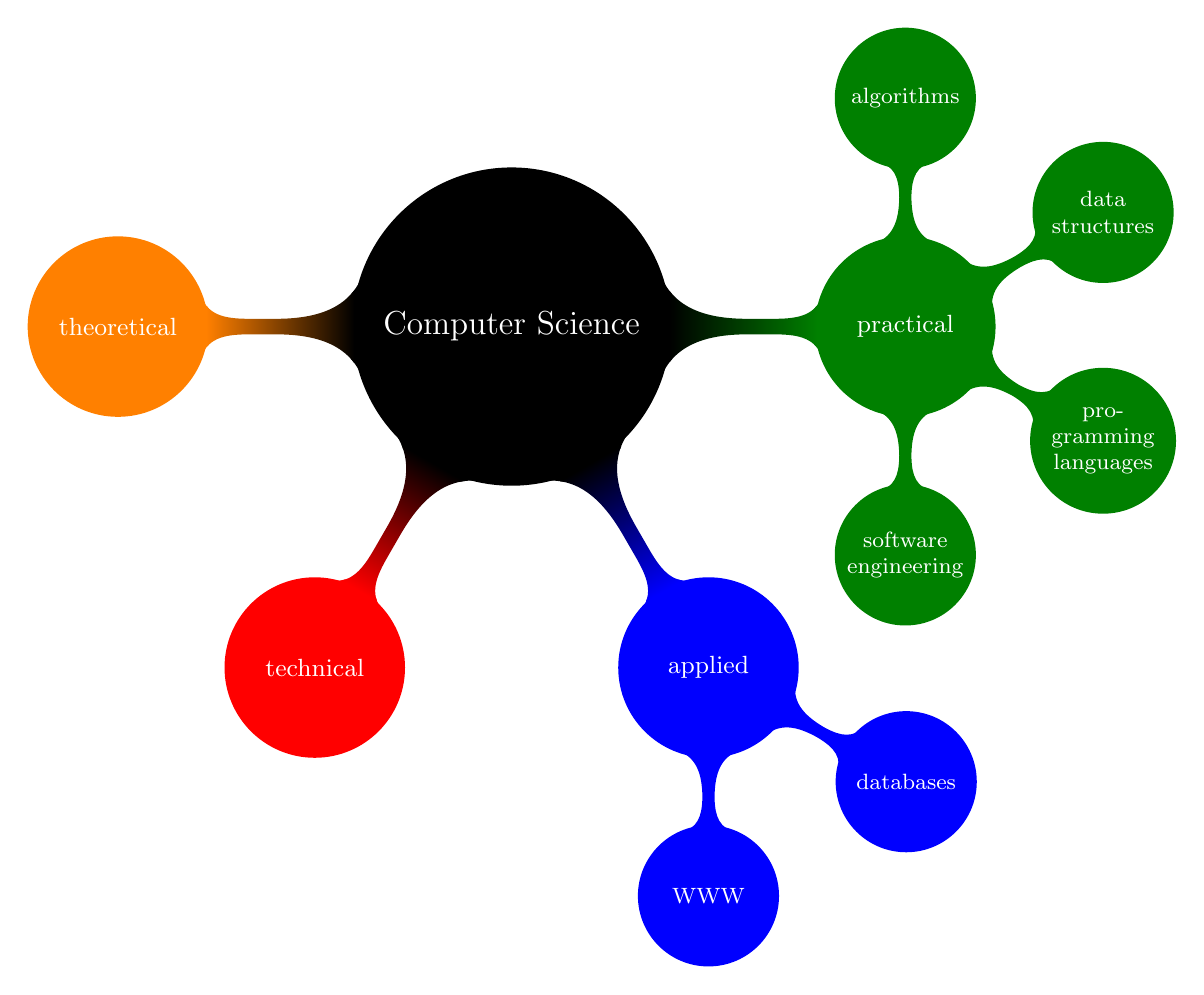
\begin{tikzpicture}
\path[mindmap,concept color=black,text=white]
node[concept] {Computer Science}
[clockwise from=0]
% note that `sibling angle' can only be defined in
% `level 1 concept/.append style={}'
child[concept color=green!50!black] {
node[concept] {practical}
[clockwise from=90]
child { node[concept] {algorithms} }
child { node[concept] {data structures} }
child { node[concept] {pro\-gramming languages} }
child { node[concept] {software engineer\-ing} }
}
child[concept color=blue] {
node[concept] {applied}
[clockwise from=-30]
child { node[concept] {databases} }
child { node[concept] {WWW} }
}
child[concept color=red] { node[concept] {technical} }
child[concept color=orange] { node[concept] {theoretical} };
\end{tikzpicture}

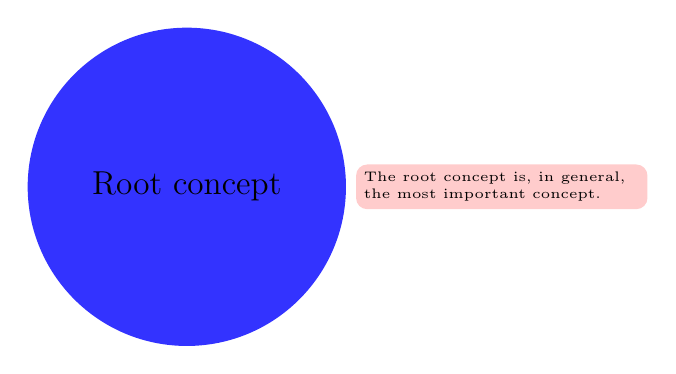
\begin{tikzpicture}
[mindmap,concept color=blue!80,
every annotation/.style={fill=red!20}]
\node [concept] (root) {Root concept};
\node [annotation,right] at (root.east)
{The root concept is, in general, the most important concept.};
\end{tikzpicture}
\end{document}
